\chapter{Results}\label{chap:results}
This chapter will present the results achieved in the project as described in Chapter \ref{chap:method}.  These results includes comparisons between different models and their hyperparameters.

\section{Analysis of the dataset}
Skriv om statisitk kring datasetet här, det som Jonatan har kollat på.

\section{The first iteration model}
The first iteration of the model was implemented with no hidden layers, as described in section \ref{sec:modelling_the_ann}. It had an LSTM-RNN layer as its input layer with 30 LSTM units. Full details on this model are found in section \ref{sec:app2_first_iter}. When this model was trained on a dataset downscaled to contain 5 users overfitting was achieved as shown in figure \ref{fig:first_iter_overfitting}.
\begin{figure}[h!]
\begin{subfigure}{0.5\textwidth}
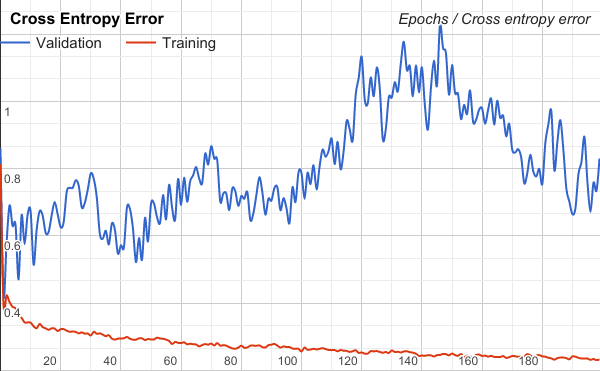
\includegraphics[width=1 \linewidth]{figure/results/first_iter_cross}
\caption{Cross entropy error}
\label{fig:first_iter_overfitting}
\end{subfigure}
\begin{subfigure}{0.5\textwidth}
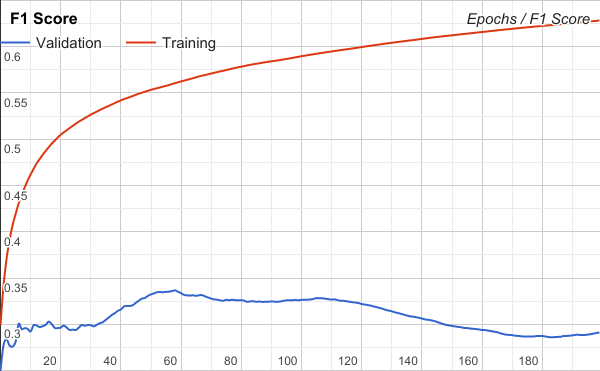
\includegraphics[width=1\linewidth]{figure/results/first_iter_f1}
\caption{$F_1$ score.}
\label{fig:first_iter_f1}
\end{subfigure}
 
\caption{The cross entropy error and $F_1$ score of the first iteration model after 200 training epochs, trained on the training and validation sets.}
\label{fig:image2}
\end{figure}
\\
The best $F_1$ score achieved on the validation set using the model was $0.3366$, as shown in figure \ref{fig:first_iter_f1}, but the main takeaway was that the model is able to learn from the data.

\section{Hyperparamaters}
The final result of the hyperparamaters are shown in table \ref{table:hyperparameters_final}

\begin{table}[h!]
    \centering
    \begin{tabular}{ r  p{7cm} }
        \hline
        \textbf{Hyperparamter}  &  \textbf{Value} \\ \hline \hline
        Learning rate & todo  \\ \hline
        Batch Size & todo \\ \hline
        RNN units & todo  \\ \hline
        Embedding Size & todo \\ \hline
        Pre-trained embedding matrix & todo \\ \hline
        Trainable embedding matrix & todo \\ \hline
        Hidden layers & todo \\ \hline
        Neurons in hidden layers & todo \\ \hline
        Usee L2 regularisation & todo \\ \hline
        L2 Factor & todo \\ \hline
        Dropout regularisation & todo\\ \hline
        Dropout probability & todo \\ \hline
        Use constant prediction limit & todo \\ \hline
        Constant prediction limit & todo  \\ \hline
        Use subreddit input & todo \\ \hline
    \end{tabular}
    \caption{Final value for all hyperparamaters}
    \label{table:hyperparameters_final}
\end{table}
\section{Baseline comparison} 
\todo{lägga in fina tabeller}
\subsection{Facebook classifier got pwned}

\subsection{Random classifier is useless}

\subsection{N-grams put up a fight}

\subsection{Highlight vector selection is not as cool as it sounds :D}


\section{Real world usability}

